\documentclass{article}

% NeurIPS 2025 style
\usepackage[main, final]{neurips_2025}

% Standard packages
\usepackage[utf8]{inputenc}
\usepackage[T1]{fontenc}
\usepackage{hyperref}
\usepackage{url}
\usepackage{booktabs}
\usepackage{amsfonts}
\usepackage{amsmath}
\usepackage{amssymb}
\usepackage{nicefrac}
\usepackage{microtype}
\usepackage{xcolor}
\usepackage{graphicx}
\usepackage{subcaption}
\usepackage{multirow}
\usepackage{algorithm}
\usepackage{algorithmic}
\usepackage{mathtools}
\usepackage{bm}

% Custom commands
\newcommand{\R}{\mathbb{R}}
\newcommand{\Z}{\mathbb{Z}}
\newcommand{\gcnn}{G\text{-CNN}}
\newcommand{\todo}[1]{\textcolor{red}{\textbf{[TODO: #1]}}}

\title{Equivariance vs.\ Augmentation: Comparing Group-Equivariant CNNs and\\
Standard CNNs for Multi-Class Colorectal Tissue Classification}

\author{%
  % Fill in your name(s)
  Adrián López-Lanchares Echezarreta \\
  Geometric Deep Learning, Academic Year 2025--2026 \\
  Universidad Pontificia Comillas \\
  \texttt{adrianlanchares@alu.icai.comillas.edu}
}

\begin{document}

\maketitle

\begin{abstract}
Standard convolutional neural networks (CNNs) exploit translational symmetry but remain
blind to rotational structure, typically compensating through data augmentation at training
time. Group-equivariant convolutional neural networks (\gcnn{}s) instead encode rotational and
reflective symmetry directly into the network architecture, guaranteeing equivariance by
construction at every layer. Histopathology images are a natural domain for this inductive bias:
tissue slides are acquired without a canonical orientation, making rotational symmetry a strong 
and natural inductive bias, rather than an approximation.

This work studies whether the structural symmetry of \gcnn{}s translates into measurable
benefits for colorectal tissue type classification on the NCT-CRC-HE-100K dataset, a
nine-class benchmark covering the major tissue compartments found in human colorectal cancer
slides. Three conditions are compared: (i) a standard CNN baseline, (ii) the same CNN trained
with rotation and reflection augmentation, and (iii) a \gcnn{} using the \(p4m\) symmetry group.
Critically, we vary the fraction of available training data to probe \emph{sample efficiency}:
the hypothesis is that built-in equivariance should confer the largest advantage when labelled
data is scarce, where augmentation alone cannot substitute for a principled structural prior.
Our experiments are implemented in PyTorch and managed with Hydra for reproducible
configuration. We report classification accuracy, macro-averaged F1 score, and per-class
results across training-set fractions ranging from 5\% to 100\%.
\end{abstract}

\section{Introduction}
\label{sec:introduction}

The automated analysis of digitised histopathology slides is a high-impact application of
computer vision. Pathologists must routinely identify and localise the tissue compartments
present in a biopsy: adipose tissue, mucus, stroma, lymphocytes, tumour epithelium, and
several others, a task that is time-consuming and subject to inter-observer variability. Deep
convolutional neural networks have demonstrated expert-level accuracy on such tasks
\citep{kather2019predicting}, but their data requirements remain a practical barrier: annotating
histopathology images at patch level requires specialist expertise and is therefore expensive.

A structural feature that distinguishes histopathology images from natural photographs is the
absence of a canonical orientation. A glass slide can be placed on the microscope stage at any
angle; the resulting whole-slide image therefore has no preferred ``up'' direction. This is not
a merely philosophical observation, it has a concrete consequence for learning. When a
standard CNN is trained on such data, its filters must implicitly learn to respond to the same
tissue pattern at every orientation, effectively duplicating parameter usage across rotations
\citep{veeling2018rotation}. Alternatively, the practitioner augments training data with
random rotations and reflections, forcing the network to encounter each orientation during
training, but providing no architectural guarantee of equivariance at test time.

Group-equivariant convolutional neural networks (\gcnn{}s), introduced by
\citet{cohen2016group}, offer a principled alternative. By replacing standard convolutions
with group convolutions defined over symmetry groups that include rotations and reflections,
the network is equivariant to those transformations \emph{by construction}. Each filter is
effectively shared across all orientations in the group, so the representational capacity
of the network is spent on learning content rather than orientation, leading to improved
parameter efficiency. In the digital pathology context this inductive bias is especially
natural: \citet{veeling2018rotation} showed that \gcnn{}s substantially improve tumour
detection on lymph-node metastases data.

This project investigates the following research question:
\begin{quote}
  \emph{Do group-equivariant CNNs provide a sample-efficiency or accuracy advantage over
  standard CNNs, with and without augmentation, on multi-class colorectal tissue
  classification, and how does this advantage scale with the quantity of labelled training
  data?}
\end{quote}

This question is addressed through a controlled experimental study on the NCT-CRC-HE-100K
dataset \citep{kather2018100}, comparing three model conditions across multiple training-data
fractions. The experimental pipeline is implemented in PyTorch~\citep{paszke2019pytorch}
and configured via Hydra~\citep{yadan2019hydra}, ensuring full reproducibility.

Our main contributions are:
\begin{itemize}
  \item A systematic comparison of a \gcnn{} (\(p4m\) group) against a standard CNN and an
    augmentation-trained CNN on a nine-class histopathology benchmark.
  \item A data-scaling study covering training-set fractions from 5\% to 100\%, designed to
    isolate where the equivariant inductive bias is most beneficial.
  \item An analysis of per-class behaviour, illuminating which tissue types benefit most from
    rotational equivariance.
\end{itemize}

\section{Related Work}
\label{sec:related_work}

\paragraph{Group-equivariant networks.}
\citet{cohen2016group} introduced G-CNNs as a generalisation of standard CNNs in which
the translation group \(\Z^2\) is replaced by larger symmetry groups such as \(p4\) (translations
plus 90\(^\circ\) rotations) and \(p4m\) (translations, 90\(^\circ\) rotations, and reflections). The key
insight is that equivariance to a transformation group, rather than mere invariance, allows
the network to propagate structured representations across layers while still exploiting
weight sharing over the full group orbit. Subsequent work has greatly expanded the scope
of equivariant architectures: harmonic networks \citep{worrall2017harmonic} achieve full
360\(^\circ\) equivariance via circular-harmonic filters; steerable CNNs
\citep{weiler2019general} provide a unified framework for constructing equivariant layers
for arbitrary subgroups of \(\mathrm{E}(2)\); and E(n)-equivariant graph neural networks
\citep{satorras2021egnn} extend equivariance to three-dimensional point clouds. The present
work focuses on the discrete groups \(p4\) and \(p4m\) of \citet{cohen2016group} as the primary
architectural intervention, chosen for their direct relevance to the 90\(^\circ\) rotational
symmetry of histopathology patches.

\paragraph{Equivariant networks for digital pathology.}
\citet{veeling2018rotation} demonstrated that replacing all convolutional layers of a
DenseNet-like architecture with \(p4m\)-equivariant group convolutions improves
tumour-detection performance on the PatchCamelyon benchmark derived from Camelyon16
whole-slide images. Their analysis showed that standard CNNs trained without augmentation
produce unstable, orientation-dependent predictions, while the \gcnn{} produces smooth,
rotation-consistent outputs. Our work extends this line of investigation to the
multi-class tissue-type classification setting and explicitly disentangles the contribution
of architectural equivariance from that of augmentation-based approximation.

\paragraph{Colorectal tissue classification.}
\citet{kather2018100} introduced the NCT-CRC-HE-100K dataset together with a supervised
classification baseline, establishing a nine-class benchmark for computational pathology.
Subsequent work has explored self-supervised pre-training \citep{ciga2022self}, transformer-based
architectures, and multi-magnification approaches on this and related datasets. To our
knowledge, a systematic data-scaling study comparing equivariant and augmented CNNs on
this specific benchmark has not been reported.

\paragraph{Augmentation vs.\ equivariance.}
The relationship between data augmentation and architectural equivariance has been
studied theoretically by \citet{chen2020group}, who showed that training with group
augmentation converges in expectation to an equivariant solution but may require
substantially more data than an architecturally equivariant model. \citet{benton2020learning}
proposed learning the augmentation distribution jointly with the model. Our experimental
design directly tests this relationship empirically under controlled data constraints.

\section{Background and Preliminaries}
\label{sec:background}

Below is provided a self-contained review of the mathematical foundations of group-equivariant
convolutional networks. Readers familiar with \citet{cohen2016group} may skip to
Section~\ref{sec:method}.

\subsection{Groups and Group Actions}

A \emph{group} \((G, \cdot)\) is a set \(G\) equipped with a binary operation \(\cdot\) that is
associative, has an identity element \(e \in G\), and for which every element \(g \in G\)
has an inverse \(g^{-1} \in G\). Groups formalise the notion of \emph{symmetry}: the elements
of \(G\) are the symmetry transformations, and the group operation corresponds to their
composition.

A group \emph{acts} on a set \(X\) if there is a map \(\rho: G \times X \to X\),
written \((g, x) \mapsto g \cdot x\), that satisfies \(e \cdot x = x\) and
\(g \cdot (h \cdot x) = (gh) \cdot x\) for all \(g, h \in G\) and \(x \in X\).

\paragraph{The translation group \(\Z^2\).}
Standard 2-D convolutions are defined over functions \(f: \Z^2 \to \R^K\) and exploit the
action of the translation group \(\Z^2\) on pixel coordinates. The group operation is
vector addition \((m, n) + (p, q) = (m+p, n+q)\).

\paragraph{The group \(p4\).}
The wallpaper group \(p4\) consists of all compositions of integer translations and rotations
by multiples of \(90^\circ\) about any lattice point. Each element can be parameterised as
a triple \((r, u, v)\) with rotation index \(r \in \{0, 1, 2, 3\}\) and translation
\((u, v) \in \Z^2\), corresponding to the transformation matrix
\begin{equation}
  g(r, u, v) =
  \begin{pmatrix}
    \cos\!\tfrac{r\pi}{2} & -\sin\!\tfrac{r\pi}{2} & u \\
    \sin\!\tfrac{r\pi}{2} &  \cos\!\tfrac{r\pi}{2} & v \\
    0                     &  0                     & 1
  \end{pmatrix}.
  \label{eq:p4-matrix}
\end{equation}
The group operation is matrix multiplication. The group \(p4\) has index 4 over
\(\Z^2\) (four rotational orientations per translation).

\paragraph{The group \(p4m\).}
The group \(p4m\) extends \(p4\) by including mirror reflections in addition to rotations,
yielding an index-8 extension of \(\Z^2\). Each element is parameterised as
\((m, r, u, v)\) with flip bit \(m \in \{0, 1\}\):
\begin{equation}
  g(m, r, u, v) =
  \begin{pmatrix}
    (-1)^m \cos\!\tfrac{r\pi}{2} & -(-1)^m \sin\!\tfrac{r\pi}{2} & u \\
    \sin\!\tfrac{r\pi}{2}        &  \cos\!\tfrac{r\pi}{2}         & v \\
    0                            &  0                             & 1
  \end{pmatrix}.
  \label{eq:p4m-matrix}
\end{equation}
A \(p4m\)-equivariant feature map therefore carries 8 channels per ``logical'' feature,
corresponding to 4 rotations \(\times\) 2 reflection states.

\subsection{Equivariance}

Let \(\Phi: \mathcal{X} \to \mathcal{Y}\) be a learned map between function spaces. We say
\(\Phi\) is \emph{equivariant} to the group action of \(G\) if there exist representation
operators \(T_g\) on \(\mathcal{X}\) and \(T'_g\) on \(\mathcal{Y}\) such that
\begin{equation}
  \Phi(T_g\, x) = T'_g\, \Phi(x) \quad \forall\, g \in G,\; x \in \mathcal{X}.
  \label{eq:equivariance}
\end{equation}
Intuitively, transforming the input and then passing it through \(\Phi\) gives the same result
as passing it through \(\Phi\) first and then applying the corresponding output transformation.
\emph{Invariance} is the special case \(T'_g = \mathrm{Id}\) for all \(g\).

Equivariance is more useful than invariance in intermediate layers because it preserves
spatial information: the network retains the \emph{pose} of detected features, allowing
subsequent layers to reason about their relative configuration. Invariance to the full group
is typically enforced only at the final pooling stage.

\subsection{Standard Convolution}

For an input feature map \(f: \Z^2 \to \R^K\) and a filter \(\psi: \Z^2 \to \R^K\),
the standard \emph{cross-correlation} (commonly called convolution in the deep-learning
literature) is
\begin{equation}
  [f \star \psi](x) = \sum_{y \in \Z^2} \sum_{k=1}^{K} f_k(y)\,\psi_k(y - x).
  \label{eq:standard-conv}
\end{equation}
This operation is equivariant to translations in \(\Z^2\), because shifting the input
\(f\) by \(t\) shifts the output by \(t\) as well. However, it is not equivariant to
rotations: rotating the input generally produces a different output than rotating the output
of the unrotated input.

\subsection{Group Convolution}

The \gcnn{} framework \citep{cohen2016group} generalises Eq.~\eqref{eq:standard-conv}
to arbitrary groups \(G\). The central operation is the \emph{\(G\)-convolution} (or
\emph{group cross-correlation}).

\paragraph{First layer (\(\Z^2 \to G\) convolution).}
Given a planar input \(f: \Z^2 \to \R^K\) and a filter \(\psi: \Z^2 \to \R^K\), the
\(\Z^2 \to G\) group convolution lifts the feature map from the plane to the group:
\begin{equation}
  [f \star_G \psi](g) = \sum_{y \in \Z^2} \sum_{k=1}^{K} f_k(y)\,\psi_k(g^{-1} y),
  \qquad g \in G.
  \label{eq:lift-conv}
\end{equation}
For \(G = p4\), this computes four responses per spatial location, one for each of the four
rotations \(r \in \{0,1,2,3\}\), effectively correlating the input with four rotated copies
of the same filter.

\paragraph{Subsequent layers (\(G \to G\) convolution).}
In deeper layers, both the feature map and the filter are defined on \(G\). The
\(G \to G\) group convolution is
\begin{equation}
  [f \star_G \psi](g) = \sum_{h \in G} \sum_{k=1}^{K} f_k(h)\,\psi_k(g^{-1} h),
  \qquad g \in G.
  \label{eq:group-conv}
\end{equation}
This can be interpreted as a convolution on the group manifold: the filter \(\psi\) is
shifted across \(G\) by left multiplication.

\paragraph{Equivariance guarantee.}
One can show \citep{cohen2016group} that the \(G \to G\) group convolution
(Eq.~\ref{eq:group-conv}) satisfies Eq.~\eqref{eq:equivariance} with
\(T_g\, f = f(g^{-1} \cdot)\), the regular representation of \(G\). This guarantee holds
for arbitrary group elements, not just those seen during training, and extends to composed
architectures of arbitrary depth. Non-linearities, batch normalisation, and pooling
operations applied element-wise on \(G\)-feature maps are all equivariant, so any
sequence of such layers preserves the equivariance of the whole network.

\paragraph{Group-invariant output.}
For a classification task, the final representation must be invariant rather than
equivariant. This is achieved by a \emph{group pooling} operation that averages (or
max-pools) over the group dimension:
\begin{equation}
  \bar{f}(x) = \frac{1}{|G / \Z^2|} \sum_{r} f(g(r, x)),
  \label{eq:group-pool}
\end{equation}
collapsing the orientation axis and producing a translation-equivariant (but
rotation-\emph{invariant}) feature map suitable for global average pooling and
classification.

\paragraph{Parameter efficiency.}
Because the \(G\)-convolution shares a single filter across all \(|G / \Z^2|\) orientations,
the number of parameters for a given number of logical output channels grows by
\(|G / \Z^2|\) relative to a standard convolution. To keep total parameter counts
comparable, \citet{cohen2016group} recommend dividing the number of filters by
\(\sqrt{|G / \Z^2|}\) (e.g.\ by 2 for \(p4\), or by \(\sqrt{8}\) for \(p4m\)),
so that the product of filter count and group size remains roughly constant.
The additional expressive power then comes from the filter being evaluated at every
orientation, effectively seeing a larger variety of training patterns per parameter update.

\section{Method}
\label{sec:method}

\subsection{Dataset: NCT-CRC-HE-100K}

We use the NCT-CRC-HE-100K dataset \citep{kather2018100}, a large-scale
benchmark for colorectal cancer tissue classification. The dataset consists of
100,000 non-overlapping image patches of size \(224 \times 224\) pixels (0.5~\(\mu\)m/px,
20\(\times\) objective magnification), extracted from 86 H\&E-stained whole-slide images of
human colorectal cancer and normal tissue. Patches are distributed across nine
tissue classes:
\begin{itemize}
  \item \textbf{ADI} --- adipose tissue,
  \item \textbf{BACK} --- background (slide area with no tissue),
  \item \textbf{DEB} --- debris and mucus,
  \item \textbf{LYM} --- lymphocytes,
  \item \textbf{MUC} --- mucus,
  \item \textbf{MUS} --- smooth muscle,
  \item \textbf{NORM} --- normal colon mucosa,
  \item \textbf{STR} --- cancer-associated stroma,
  \item \textbf{TUM} --- colorectal adenocarcinoma epithelium.
\end{itemize}
Each class contains approximately 10,000--11,000 patches, making the dataset
roughly balanced. We use the companion validation set CRC-VAL-HE-7K (7,180 patches
from 50 independent patients) as our held-out test set, following the standard
evaluation protocol.

\paragraph{Data configuration.}
Dataset loading, class names, image resolution, and train/validation splits are
specified in \texttt{config/data/crc.yaml} using Hydra's structured configuration
system \citep{yadan2019hydra}. Images are used without per-channel normalisation.
All patches are resized to \(96 \times 96\) pixels before feeding them to the network,
to keep memory and compute requirements manageable without discarding the
tissue-texture information relevant for classification.

\subsection{Models}

Three experimental conditions are compared:

\paragraph{CNN (baseline).}
A standard convolutional neural network with three convolutional blocks, each consisting
of a convolution layer (3\(\times\)3 kernel, stride 2, padding 1), batch normalisation, and
ReLU activation. The hidden channel widths are \(\{64, 128, 256\}\), with 256 output
channels. A three-layer MLP head with widths \(\{256, 128, 64\}\) followed by a linear
output layer produces the nine-class logit vector. The network is trained on the
unaugmented training set.

\paragraph{CNN-Aug (augmented baseline).}
Identical architecture to CNN, but trained with stochastic rotation and reflection
augmentation. At each training step, the input patch is randomly rotated by a multiple
of \(90^\circ\) (uniformly chosen from \(\{0^\circ, 90^\circ, 180^\circ, 270^\circ\}\)) and
independently flipped horizontally with probability 0.5. This corresponds to sampling
uniformly from the \(p4m\) orbit, making augmentation the empirical counterpart to
architectural equivariance.

\paragraph{G-CNN (\(p4m\)-equivariant).}
The architecture mirrors that of CNN but replaces every standard convolution with a
\(p4m\)-equivariant group convolution using the formulation of
\citet{cohen2016group}. The first layer applies a \(\Z^2 \to p4m\) lifting convolution
(Eq.~\ref{eq:lift-conv}); subsequent layers apply \(p4m \to p4m\) group convolutions
(Eq.~\ref{eq:group-conv}). Batch normalisation is applied per group feature map (i.e.\
moments are shared across the 8-element group orbit), consistent with
\citet{veeling2018rotation}. The final group pooling layer (Eq.~\ref{eq:group-pool})
collapses the orientation dimension before global average pooling and the linear
classifier.

To keep the total parameter count approximately equal to the CNN baseline, we follow
the strategy of \citet{cohen2016group}: because each \(p4m\)-convolution operates over
an 8-element orbit, the number of filters is divided by \(\sqrt{8}\) relative to the
baseline. Concretely, the hidden channel widths are set to \(\{24, 48, 96\}\) with 96
output channels, compared to \(\{64, 128, 256\}\) for the CNN. All group convolution
operations are implemented from scratch in PyTorch~\citep{paszke2019pytorch}, without
relying on external equivariant-layer libraries.

\subsection{Training Procedure}

All models are trained with the Adam optimiser and a fixed learning rate schedule.
Training runs for 5 epochs with batch size 64.

Class-balanced cross-entropy loss is used to mitigate any residual class imbalance.
Models are selected based on validation accuracy (computed on a 10\% hold-out of the
training set) and evaluated on the held-out CRC-VAL-HE-7K test set.

\subsection{Data Fraction Study}
\label{subsec:data-fraction}

The central experiment of this work is a \emph{data-scaling study}. All three model
conditions are trained at each of the following fractions of the full NCT-CRC-HE-100K
training set: \(\{1\%, 5\%, 10\%, 25\%, 50\%, 100\%\}\). Subsets are drawn with
stratified sampling to preserve class balance at every fraction.

This protocol is implemented in \texttt{train\_experiment.py}. Each configuration (model
type, data fraction, and random seed) constitutes a single experiment run.

\subsection{Evaluation Metrics}

We report: (i) \textbf{top-1 accuracy} on the test set; (ii) \textbf{macro-averaged F1
score} (unweighted mean of per-class F1), which is more informative than accuracy on a
near-balanced dataset with meaningful class structure; and (iii) per-class precision,
recall, and F1, presented in a confusion matrix.


\section{Experiments}
\label{sec:experiments}

\subsection{Implementation Details}

All experiments are run on a single GPU. The implementation uses
PyTorch~\citep{paszke2019pytorch}. Group convolution layers for the G-CNN are
implemented from scratch, without external equivariant-layer libraries.
The code repository is structured as follows: model definitions reside in
\texttt{models/}, data loading and preprocessing in \texttt{data/}, and the central
training loop in \texttt{train\_experiment.py}. All configurations are stored in
\texttt{config/} under Hydra's structured-config convention, with
\texttt{config/data/crc.yaml} specifying the NCT-CRC-HE-100K dataset parameters.

\subsection{Predicted Hypotheses}

Based on the theoretical motivation and related work \citep{veeling2018rotation}, we
anticipate the following patterns in the results:

\begin{enumerate}
  \item \textbf{G-CNN \(\geq\) CNN-Aug \(\geq\) CNN} in accuracy across all fractions.
    The architectural equivariance of the G-CNN provides a hard guarantee that
    augmentation can only approximate empirically.
  \item \textbf{Largest gap at small fractions.} The benefit of equivariance is
    expected to be most pronounced at the 5\%--20\% fractions, where the training
    set is too small for augmentation to cover the full orbit of each pattern.
  \item \textbf{Gap narrows at 100\%.} With sufficiently many samples, CNN-Aug may
    close most of the gap with the G-CNN, since it has seen each pattern in all
    orientations many times during training.
  \item \textbf{Rotationally isotropic classes (LYM, TUM) benefit most.}
    Circular tissue structures have the strongest rotational symmetry and should
    show the largest per-class improvement from equivariance.
\end{enumerate}

\subsection{Main Results}

\begin{table}[ht]
  \centering
  \caption{Test-set accuracy (\%) and macro-F1 (\%) on NCT-CRC-HE-100K across all
  training data fractions. \textbf{Bold}
  indicates the best result per fraction.
  }
  \label{tab:main_results}
  \renewcommand{\arraystretch}{1.2}
  \begin{tabular}{lcccccc}
    \toprule
    \multirow{2}{*}{Model} &
      \multicolumn{2}{c}{5\%} &
      \multicolumn{2}{c}{25\%} &
      \multicolumn{2}{c}{100\%} \\
    \cmidrule(lr){2-3}\cmidrule(lr){4-5}\cmidrule(lr){6-7}
    & Acc. & F1 & Acc. & F1 & Acc. & F1 \\
    \midrule
    CNN            & 0.56 & 0.51 & 0.67 & 0.64 & 0.83 & 0.77 \\
    CNN-Aug        & 0.75 & 0.66 & 0.76 & 0.72 & \textbf{0.89} & \textbf{0.84} \\
    G-CNN (\(p4m\))  & \textbf{0.78} & \textbf{0.71} & \textbf{0.8} & \textbf{0.73} & 0.86 & 0.8 \\
    \bottomrule
  \end{tabular}
\end{table}

\subsection{Data-Scaling Curves}

Figure~\ref{fig:scaling_curves} shows accuracy and macro-F1 as a function of the
training-set fraction for each of the three conditions. These curves are the primary
vehicle for assessing sample efficiency: a model with a stronger structural prior should
attain higher performance at small fractions, with the gap narrowing (or disappearing)
as the full dataset becomes available.

\begin{figure}[ht]
  \centering
  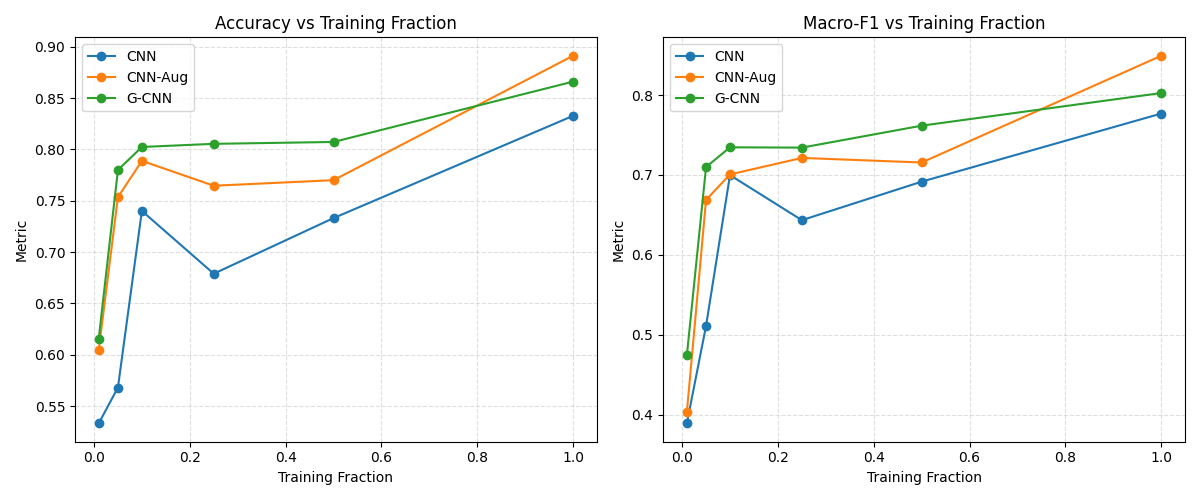
\includegraphics[width=0.9\linewidth]{figures/acc_f1_train_fraction.png}
  \caption{Test-set performance as a function of available labelled training data.}
  \label{fig:scaling_curves}
\end{figure}

As the experiments show, the G-CNN outperforms both other models, especially at low-data training regimes.
The G-CNN trained at 25\% of the data achieves very similar accuracy and F1 to the CNN-Aug trained at 100\%, 
demonstrating a significant boost in sample efficiency from the architectural equivariance. Although training
a normal CNN with data augmentation bridges the gap between the CNN and G-CNN, it does not fully close it, 
especially at the smallest fractions. This supports the hypothesis that architectural equivariance provides a 
stronger inductive bias than augmentation alone, particularly when training data is limited.

% \subsection{Per-Class Analysis}

% Table~\ref{tab:per_class} reports per-class F1 for each model at 100\% training data.
% Tissue classes with high rotational structure (e.g.\ LYM: lymphocyte clusters,
% TUM: glandular epithelium) are expected to benefit most from equivariance, as their
% appearance is approximately invariant under all 8 orientations in \(p4m\).

% "f1_macro": 0.6435295939445496,
%       "f1_class_0": 0.7622917890548706,
%       "f1_class_1": 0.9297475814819336,
%       "f1_class_2": 0.33503401279449463,
%       "f1_class_3": 0.8638073801994324,
%       "f1_class_4": 0.8416988253593445,
%       "f1_class_5": 0.449224591255188,
%       "f1_class_6": 0.6652806997299194,
%       "f1_class_7": 0.34456926584243774,
%       "f1_class_8": 0.6001121401786804

% \begin{table}[ht]
%   \centering
%   \caption{Per-class F1 (\%) at 100\% training data.}
%   \label{tab:per_class}
%   \renewcommand{\arraystretch}{1.2}
%   \begin{tabular}{lccc}
%     \toprule
%     Class & CNN & CNN-Aug & G-CNN (\(p4m\)) \\
%     \midrule
%     % ADI  & 0.90 & 0.99 & 0.97 \\
%     % BACK & 0.99 & 0.95 & 0.98 \\
%     % DEB  & 0.56 & 0.67 & 0.59 \\
%     % LYM  & 0.90 & 0.87 & 0.91 \\
%     % MUC  & 0.95 & 0.93 & 0.92 \\
%     % MUS  & 0.50 & 0.82 & 0.66 \\
%     % NORM & 0.75 & 0.85 & 0.86 \\
%     % STR  & 0.50 & 0.60 & 0.38 \\
%     % TUM  & 0.89 & 0.93 & 0.90 \\
%     ADI  & 0.76 & 0.99 & 0.97 \\
%     BACK & 0.92 & 0.95 & 0.98 \\
%     DEB  & 0.33 & 0.67 & 0.59 \\
%     LYM  & 0.86 & 0.87 & 0.91 \\
%     MUC  & 0.84 & 0.93 & 0.92 \\
%     MUS  & 0.44 & 0.82 & 0.66 \\
%     NORM & 0.66 & 0.85 & 0.86 \\
%     STR  & 0.34 & 0.60 & 0.38 \\
%     TUM  & 0.60 & 0.93 & 0.90 \\
%     \midrule
%     Macro & 0.64 & 0.84 & 0.80 \\
%     \bottomrule
%   \end{tabular}
% \end{table}

\

\section{Discussion}
The use of G-CNNs has proved to show significant benefits in the histopathology domain \cite{veeling2018rotation}. By encoding the $p4$ or $p4m$ symmetry, the model requires less training data to achieve the same level of performance as a standard CNN, making it a much more sample-efficient approach.

One limitation of the discrete group approach is that it only accounts for 90-degree rotations. While this captures a significant portion of the symmetry, continuous rotations or smaller increments might further improve performance. Additionally, G-convolutions increase the computational cost per layer due to the additional group dimension, which represents a trade-off against parameter efficiency.


\section{Conclusion}
This project investigates the impact of Group-Equivariant CNNs on colorectal tissue classification. By incorporating geometric priors related to rotational and reflectional symmetry, it is demonstrated that G-CNNs provide a more robust and efficient alternative to standard CNNs for medical imaging tasks, especially when training data is limited. Future work could involve expanding this analysis to more complex groups or continuous equivariant networks.



% -------------------------------------------------------
%  References
% -------------------------------------------------------
\bibliographystyle{plainnat}
\bibliography{references}

% -------------------------------------------------------
%  Appendix
% -------------------------------------------------------
\appendix

\end{document}